\section{Technology selection rationale}

The selection of the Tino V2 technology stack followed a requirements-driven process that balanced perception accuracy, real-time constraints on embedded hardware, integration complexity with legacy code, and operational robustness for prolonged experiments. The priorities used to evaluate candidate technologies were:

\begin{itemize}
	\item \textbf{Functional accuracy}: localization and human pose estimation must be precise enough to feed the VR system with metric robot pose and 3D human joint positions.
	\item \textbf{Real-time performance}: the chosen algorithms must run on the onboard computer (NVIDIA Orin Nano) with low latency to satisfy VR and teleoperation requirements (target end-to-end perception latency $<$ 100 ms where possible).
	\item \textbf{Integration and maintainability}: preference for solutions with ROS2 support, stable persistence (map save/load and relocalization), and reasonable build effort on ARM64.
	\item \textbf{Robustness and recoverability}: the system must tolerate temporary sensor dropouts, relocalize from different viewpoints, and provide fallbacks to reduce mission-critical failures.
\end{itemize}

Using these criteria, the final choices were: RTABMap for SLAM and map management, an Oak-D Pro (DepthAI) stereo camera for visual + depth input, UWB anchors for absolute positioning, and a YOLOv11-based pose estimation pipeline accelerated with TensorRT for real-time skeleton extraction. The justifications are summarised below.

\begin{figure}[H]
	\centering
	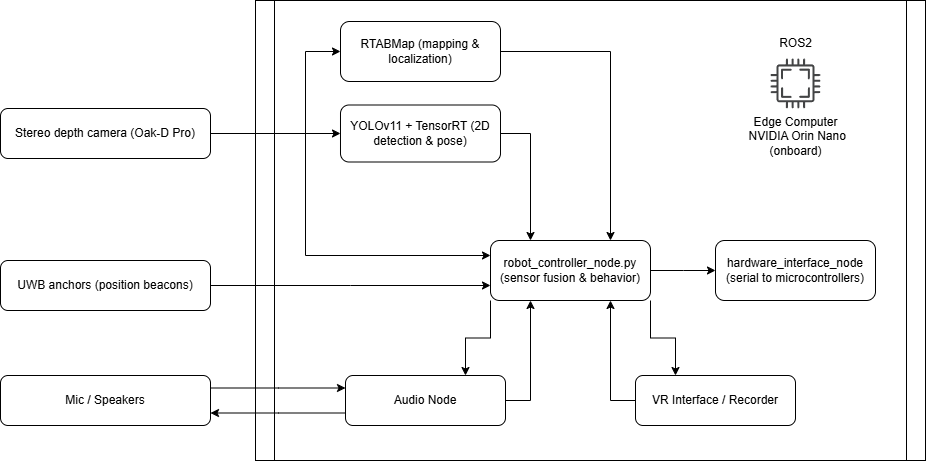
\includegraphics[width=0.85\linewidth]{Images/system_architecture.png}
	\caption{High-level system architecture for Tino V2.}\label{fig-system-architecture}
\end{figure}

\subsection*{Why RTABMap over ORB‑SLAM3 and SVO}
RTABMap provides robust multi-session map persistence, reliable relocalization and first-class ROS/ROS2 integration. During early experiments ORB‑SLAM3 and SVO presented compilation fragility on ARM64 and unstable atlas save/load behavior with the available cameras. RTABMap demonstrated stable map saving/loading and dependable relocalization in practice, making it preferable for a system where map reuse and long-term experiments are required.

\subsection*{Why Oak‑D Pro and DepthAI}
The Oak‑D Pro was chosen because it provides synchronized stereo depth and on‑device compute options while integrating well with the DepthAI stack and ROS2 wrappers. The camera proved reliable in mapping and provided stereo depth required to convert 2D detections into metric 3D positions.

\subsection*{Why UWB}
UWB anchors provide absolute positioning that compensates SLAM drift and long‑run integration error. When fused with visual SLAM, UWB supplies global corrections and increases robustness in feature‑poor or dynamic areas where visual relocalization is unreliable.

\subsection*{Why YOLOv11 + TensorRT}
YOLOv11, converted to TensorRT engines, provided the best trade-off between detection accuracy and inference throughput on the Orin Nano. The pipeline was extended to extract 17-joint skeletons and fuse per-joint depth from the Oak‑D stereo stream to produce metric 3D skeletons suitable for VR avatars.

\subsection*{R\&D chronology and selection summary}
During development multiple SLAM and VO approaches were evaluated. ORB‑SLAM3 was tested first for its academic strengths and multi‑sensor support, but proved fragile to compile and unstable with the available cameras on ARM64. SVO was attempted as a lighter‑weight alternative but exhibited similar portability and map‑management limitations. RTABMap paired with the Oak‑D Pro ultimately provided the reliable map persistence, dependable relocalization and ROS2 interoperability required for repeated experimentation, and was therefore adopted as the primary mapping solution for Tino V2.

\section{Hybrid localization strategy}

The localization architecture is intentionally hybrid: RTABMap supplies dense map information and orientation (visual odometry and loop closures) while UWB supplies absolute position corrections. The approach follows an architecture with three functional layers:

\begin{enumerate}
	\item \textbf{Sensor acquisition layer:} Oak‑D stereo frames, depth images, RTABMap odometry, UWB range fixes, and IMU measurements are published on ROS2 topics.
	\item \textbf{Local estimation layer:} RTABMap performs visual odometry and graph optimization, producing local pose estimates and maps. Short-term pose updates come from visual odometry and IMU fusion where available.
	\item \textbf{Global fusion layer:} a fusion node ingests RTABMap pose and UWB positions and performs simple sensor selection logic that maintains a consistent global pose used by the rest of the system (VR exporter, motion controller, logging).
\end{enumerate}

This structure leverages RTABMap's strength in building and maintaining appearance-based maps and UWB's absolute fixes to constrain long-term drift. In the Tino V2 implementation the global fusion logic is implemented inside the \texttt{robot\_controller\_node}: it ingests RTABMap poses, UWB fixes, IMU deltas and performs simple sensor selection and fallback logic before publishing the consolidated \texttt{localization\_pose} topic consumed by the VR bridge and other consumers.

\begin{figure}[H]
	\centering
	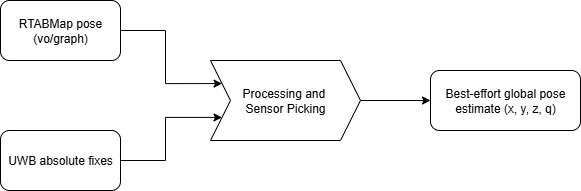
\includegraphics[width=0.85\linewidth]{Images/sensor_fusion.png}
	\caption{Sensor selection and dataflow.}\label{fig-sensor-fusion}
\end{figure}

\subsection*{Sensor fusion contract}
\begin{description}
	\item[Inputs:] RTABMap pose (x, y, z, q), UWB position fixes (x, y, timestamp), IMU measurements (angular velocity, linear acceleration). All inputs are timestamped and published on ROS2 topics.
	\item[Outputs:] A best-effort global pose estimate (x, y, z, q) selected from available sensors; the node republishes the fused pose at a variable rate (typically 10--50\,Hz depending on sensor availability and computational load).
	\item[Error modes:] \begin{itemize}[nosep,leftmargin=*]
		\item \textbf{Missing UWB fixes:} the fusion falls back to visual odometry from RTABMap.
		\item \textbf{Visual tracking loss:} the system holds the last known map pose and uses UWB position with estimated orientation from movement direction; if unsuccessful, it raises an operator-visible warning.
		\item \textbf{Inconsistent UWB readings:} basic validity checks are applied and the system falls back to RTABMap position when UWB appears invalid.
	\end{itemize}
\end{description}

\subsection*{Edge cases and mitigations}
\begin{itemize}
	\item \textbf{NLOS UWB measurements:} detect through basic position validation checks; rely on RTABMap until UWB stabilizes.
	\item \textbf{Feature-poor areas (e.g., blank walls):} increase re-scan or operator-triggered relocalization.
	\item \textbf{Camera occlusion by robot fabric:} use stereo depth fallback and restrict robot motion until visual lock is recovered.
\end{itemize}

\section{Human detection and pose pipeline}

The human perception pipeline is designed to provide real-time 3D skeletons to the VR environment and other behavior nodes. It consists of three stages:

\begin{enumerate}
	\item \textbf{2D detection and pose estimation:} YOLOv11 (TensorRT engine) runs on RGB frames to detect humans and estimate 2D keypoints (17 joints).
	\item \textbf{Depth association:} for each detected joint, the pipeline samples the Oak‑D stereo depth (with median filtering in a small neighbourhood) to recover the joint's metric z coordinate and compute the (x,y,z) position in the camera frame.
	\item \textbf{Transform to robot/world frame:} the 3D joint positions are transformed using the current fused global pose to provide world-relative skeleton's coordinates for VR and navigation.
\end{enumerate}

\begin{figure}[H]
	\centering
	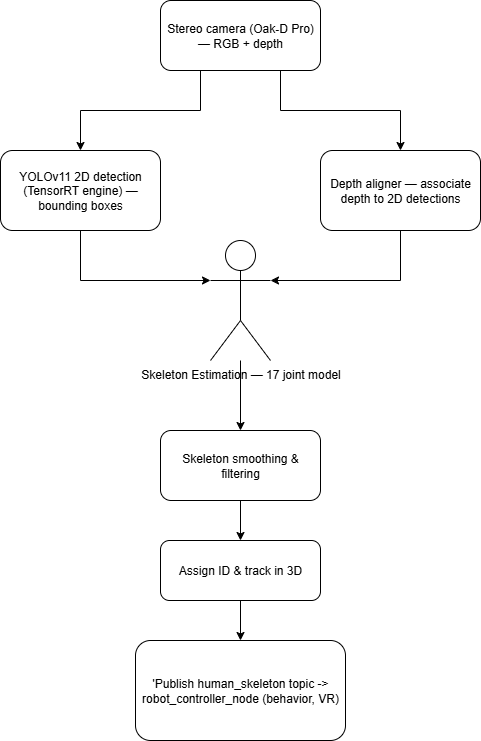
\includegraphics[width=0.85\linewidth]{Images/human_pipeline.png}
	\caption{Human detection and depth-association pipeline.}\label{fig-human-pipeline}
\end{figure}

The pipeline publishes a \texttt{human\_skeleton} ROS2 message containing a timestamped array of joints, each with position and a confidence score. This message enables downstream nodes to select stable skeletons for interaction logic and VR rendering.

\subsection*{Design contract for perception}
Inputs: synchronized RGB frame, depth image, camera intrinsics, current global pose.
Outputs: timestamped skeletons with 3D joint positions and per-joint confidence.
Failure modes: low confidence joints (reported but flagged), missing depth (use last known depth or drop joint), multiple detections (assign IDs using bounding-box IoU + temporal tracking).

\section{Software architecture and system organisation}

To improve modularity and maintainability the entire robot stack was migrated to ROS2. The project uses a node-based split that mirrors the functional decomposition:

\begin{itemize}
	\item \textbf{Perception:} \texttt{rtabmap} (mapping/localization), \texttt{depthai} camera node, \texttt{yolo11\_pose\_node} (TensorRT inference + skeleton extraction).
	\item \textbf{State and logging:} \texttt{vr\_data\_recorder\_node} (logging for VR and experiments).
	\item \textbf{Control (includes fusion):} \texttt{robot\_controller\_node.py} implements simple sensor selection logic (UWB preferred for position, RTABMap for orientation) and high-level behaviours; \texttt{hardware\_interface\_node.py} handles serial comms to Arduinos using device symlinks \texttt{/dev/ttyHEAD}, \texttt{/dev/ttyBASE}, \texttt{/dev/ttyLEG}.
	\item \textbf{I/O and integration:} \texttt{gamepad\_node.py}, \texttt{audio\_node.py}, \texttt{vr\_interface\_node.py} (VR bridge and topic translation).
\end{itemize}

Design decisions that improved robustness during development included using persistent device symlinks for Arduinos, clearly separated launch files for mapping and localization (\texttt{rtab\_mapping.launch.py}, \texttt{rtab\_localization.launch.py}), and a dedicated VR exporter node that limits published bandwidth and enforces message rate caps for stable VR telepresence.

\section{Implementation notes and rationale from R\&D}

Several practical findings from the development period informed the conceptual choices:

\begin{itemize}
	\item ORB‑SLAM3 and SVO showed compilation and stability problems on ARM64 devices and with older RealSense/T265 hardware; this motivated the switch to RTABMap and the Oak‑D Pro camera.
	\item The Oak‑D Pro + RTABMap standalone build achieved reliable map save/load and relocalization, a key requirement for repeated VR sessions.
	\item Converting YOLOv11 to TensorRT produced the necessary runtime performance for 17-joint skeleton extraction on the Orin Nano while keeping end-to-end latency acceptable for virtual reality.
	\item Power architecture and mechanical changes (new differential base, improved mounts for camera and speakers) reduced vibration and improved perception robustness in the field.
\end{itemize}

\section{Validation plan and quality gates}

To verify the conceptual choices and measure system readiness the following minimal quality gates were defined and executed where possible:

\begin{enumerate}
	\item \textbf{Build and integration:} RTABMap + DepthAI + ROS2 launch files must start and publish \texttt{localization\_pose} and camera topics without crashes for 10 minutes (smoke test).
	\item \textbf{Perception correctness:} YOLOv11 TensorRT skeletons validated against recorded test sequences; per-joint reprojection error to depth must be within 20 cm for frontal poses.
	\item \textbf{Fusion stability:} sensor selection logic must provide reasonable pose estimates when UWB anchors are available, and be able to relocalize to saved maps.
	\item \textbf{End-to-end latency:} perception -> VR message latency measured and kept below 150 ms in typical configurations.
\end{enumerate}

Measured results from the R\&D include:
\begin{itemize}[nosep]
	\item RTABMap with Oak‑D saved and reloaded maps reliably.
	\item YOLOv11 (TensorRT) provided real-time skeletons suitable for VR export.
	\item Orin Nano peak current draw was measured and verified as acceptable after power supply revisions.
\end{itemize}

\section{Summary}

This chapter formalises the conceptual choices behind Tino V2: a ROS2-centred architecture using RTABMap for mapping, Oak‑D Pro for stereo depth, UWB for absolute positioning, and a YOLOv11+TensorRT pipeline for real-time human pose estimation. The chosen sensor selection approach balances metric accuracy, runtime performance and practical robustness demonstrated during the development phase.

